\documentclass[12pt,pdftex]{article}
\usepackage{amsmath}
\usepackage{graphicx}
\usepackage{natbib}
\citestyle{elsart-harv}
\usepackage{rotating}
\usepackage{lineno} 
\usepackage{longtable}
\usepackage{amsmath}
\usepackage{amssymb}
\usepackage{subcaption}

% Text layout
\topmargin 0.0cm
\oddsidemargin 0.5cm
\evensidemargin 0.5cm
\textwidth 16cm 
\textheight 21cm

% Leave date blank
\date{}

\title{Conditions for successful range shifts}
                                                                  
\author{Jonatan \r{A}revall$^{1}$,  Regan Early$^{2}$, Alba Estrada$^{3}$, \\ Uno Wennergern$^{1}$ \& Anna Ekl\"{o}f$^{1*}$,\\
  $^1$\small Department of Physics, Chemistry and Biology, Division of Theoretical Biology, Sweden\\
  $^2$\small Centre for Ecology and Conservation, University of Exeter Penryn Campus, Cornwall, UK\\
 $^3$\small Department of Animal Biology, University of M\`{a}laga, Campus de Teatinos, Spain.\\
  $^*$ \small Corresponding author: anna.eklof@liu.se\\
}
\begin{document}
\linenumbers
\maketitle
\baselineskip 18pt

\subsubsection*{Corresponding author}
Anna Ekl\"{o}f\\
Link\"{o}ping University\\ 
Department of Physics, Chemistry \& Biology\\
Division of Theoretical Biology
Link\"{o}ping, SWEDEN\\

\noindent {\bf Running title:} 

\noindent {\bf Number of words:} 

\clearpage

% Please keep the abstract at maximum 300 words
\begin{abstract}
max 300 words
\end{abstract}

\noindent {\bf Key words:} 
climate change, range shift, landscape configuration, point pattern
\section*{Abstract}
Ongoing climate change is currently modifying the geographical location of areas that are climatically suitable for species’. Understanding a species ability to successfully shift their geographical range, performing a range shift, have important implications for assessing extinction risks and predicting future community compositions. Here we model how a species' ability to track a directional shift in climatic conditions is affected by: i) species dispersal abilities; ii) speed of climatic shift; and iii) spatial arrangement of the habitat. Our modeling framework includes within- and between patch population dynamics and use ecologically realistic habitat distributions and dispersal scenarios, and, as such, is an extension and improvement of classical range shift models.

We show that all three factors have clear effects on the density and persistence of local populations following a climatic shift. In particular we show that it is not solely the amount of habitat that is of importance, but rather the actual distribution of the patches of suitable habitats. Additionally, a species dispersal pattern has profound effects on their success on colonizing new habitats, and the outcome is tightly linked to the speed of the climatic shift. This points out the importance of taking the interplay of a species dispersal and the landscape configuration into account when estimating future climate impact on species. These results link ecologically important attributes of both species and their landscapes to outcomes of species range shift, and thereby long-term persistence of ecological communities. 



\clearpage

\section*{Introduction}
One of the most important factors for how species are distributed around the globe is their tolerance of climatic conditions \citep{Thomas2010}. However, ongoing climate change is currently changing location of the areas that are climatically suitable for species’ \citep{Loarie2009}, and there is clear evidence that these changes indeed are inducing shifts in latitudinal distributions for a wide variety of organisms \citep{Parmesan2003, Chen2011,Lenoir2015}. However, there are also several examples where species have not been able to track the changes in climatic conditions \citep{Maclean2011}  and thereby facing the risk of eventually going extinct. Therefore species' capabilities of successfully tracking the changing climate have far-reaching consequences for biodiversity \citep{Thuiller2005a}. 

For most ecosystems around the world habitat loss, degradation and fragmentation are primary causes of species declines \citep{Fahrig2003, JoernFischer2006}. Climate change is predicted to increasingly interact with, and often intensify, the effects of these factors \citep{Doerr2011}. Ultimately, the survival of a population, facing a changing climate, depends on its ability to either adapt to the new conditions \citep{Hoffmann2011,Sentis2015} or successfully disperse and colonize new geographical areas \citep{Travis2013}.  Understanding of how species distributions and persistence are likely to be affected by climate change, in combination with factors affecting dispersal and colonization success, is critical to inform effective conservation strategies in a changing world \citep{Gillson2013a}. 

Landscapes, natural as well as human-modified, can be viewed as geographical areas scattered with suitable and unsuitable habitats combined in different densities and configurations. Since species dispersal is a process that links discrete habitat patches together and not only the amount of habitat is important for a successful dispersal event, but also the actual distribution of the habitat patches in the landscape \citep{Villard1999, Baguette2013}. In fragmented landscapes the amount of habitat and landscape connectivity are often linked to each other \citep{Villard2014} but the relationship is by no means a necessity \citep{Wang2014} as the same amount of habitat can be distributed in various ways and thereby give different degrees of structural connectivity in the landscape. When the landscape gets re-structured due to land-use modifications, e.g., becomes more fragmented, the negative effects of lower structural connectivity is especially pronounced for species with certain characteristics, such as strong adaptation to the historic landscape configuration or low dispersal ability \citep{Brook2016}. Climate change may in turn cause both habitats and the matrix decrease in quality \citep{Martin2016}, potentially giving catalyst effects between land-use and climate change \citep{Pielke2005}. The landscape configuration, the species dispersal ability, and quality of the new habitat jointly contribute to the realized connectivity (how structural connectivity is experienced by the species) and ultimately determines the outcome of species dispersal \citep{Baguette2013, Borthagaray2014}. 

%For the dispersing individuals there is often a risk coupled to the dispersal events \citep{Cowen2000a, Eklof2012b}, due to for example matrix with lower quality between high-quality habitat patches \citep{Gaines1980} or landscape barriers limiting dispersal into suitable habitats \citep{Opdam2004}. 

Species abilities to track a changing climate is additionally dependent on how fast the climatic shift is progressing \citep{Schloss2012a}, and there can be profound differences in speed of change between biomes \citep{Stocker2013, Loarie2009}. Potentially species that are able to disperse at a fast pace should have better prerequisites to track a fast shift in climatic conditions compared to a species with slower dispersal rate \citep{Walther2002, Angert2011}, with implications for biodiversity and other features of community structure. 

Predicting biodiversity scenarios under climate change has so far to large extent relied on species distribution models, SDM, \citep{Guisan2000, Thomas2006a}, where  the statistical correlations between current species distribution and a set of environmental variables are used to do predictions of future distributions. However, the accuracy of these models to deliver reliable predictions have been extensively discussed \citep{Thuiller2013, Araujo2012a, Wiens2009} owing to limitations such as species dispersal often considered unlimited or non-existent \citep{Peterson2001, Thuiller2005a} and exclusion of population dynamics \citep{Zurell2009}. To meet this limitations there has been a recent development of ``hybrid models'', which combine the classical SDM approach with, for example, simple dispersal or population dynamic models \citep{Ehrlen2015}. \cite{Zurell2016} recently tested the predictive performance of  models for range dynamics differing in their complexity, and concluded a clear advantage for models including dynamic approaches. 

To reliably predict range dynamic in the face of climate change we need to understand the joint impact of species’ dispersal, habitat configuration in landscapes and speed of climatic shift on species abilities to colonize and survive in new climatically suitable areas. Simulations of virtual landscapes/species can be highly informative but typically face several limitations. They typically focus on population presence/absence, rather than measuring population growth and abundance and typically lack ecological realism. To this extent we here develop a modeling framework for species range shifts %including three key aspects by: 1) explicitly include population dynamics in the model, 2) evaluate different types of habitat configuration within landscapes, and 3) use data on dispersal kernels and speed of climate change for real species and landscapes. 
where we include two improvements – to include carrying capacity and population growth rates in the model, and to use data on dispersal kernels and speed of climate change for real species and landscapes when evaluating different types of habitat configurations.

\section*{Materials and Methods}

We model how species' ability to track a directional shift in climatic conditions is affected by i) spatial arrangement of suitable habitats in the landscape, ii) characteristics of the species dispersal abilities and iii) speed of the climatic shift. We explore the effect these factors have on the migrating population in terms of patch occupancy and changes local and global density. To as large extend as possible we use empirical data to justify the choice of parameter values in our model.

\subsection*{Landscape generation}
We start by producing a set of artificial landscapes varying in their configuration of suitable habitat patches.We specifically want to analyze landscapes with a clear difference in habitat aggregation. To this extent we follow a recently developed methodology \citep{Lindstrom2011}, where the landscapes are generated using a method based on spectral density to produce neutral point pattern landscapes (NPPL). The NPPLs are primarily defined by three parameters: the number of patches ($n$ß), a continuity parameter ($\gamma$) and a contrast parameter ($\delta$). The continuity parameter determines the spatial autocorrelation over multiple scales, i.e., if areas with similar patch density are located close to or far from each other. The contrast parameter defines how large the difference between dense and sparse areas is, i.e., is a measure of density dispersion. For a detailed description of the method see \cite{Lindstrom2011}.

%We here want to generate landscapes that varies in habitat aggregation.
% we initially used three different values of $\gamma$ and $\delta$: 1,3 and 5, and 0, 1 and 2 respectively.  This gives in total seven different landscape configurations (as landscapes with high  γ and low δ  is not possible). We produce 30 replicates of each landscape type. 
We here we vary $\gamma$ but keep $\delta$ constant. The combinations used are [$\gamma$=0, $\delta$= 3] and [$\gamma$=2, $\delta$= 3] as those represent landscapes with a clear difference in habitat aggregation (see Fig. 1 for an example landscapes). We hereafter refer to those combinations as homogeneous and heterogeneous landscapes respectively. The number of habitat patches distributed in each landscape is 1000.

In order to evaluate the ecological relevance of the generated landscapes we compare them to empirical data. The empirical data used here describe the distribution of suitable habitats after climate change for the European mammal species used to justify the dispersal kernels  (see SI).  We compare the aggregation of suitable habitat in the simulated and empirical landscapes using the Clark and Evans aggregation index \citep{Clark1954}. This comparision gives a rough estimate of the spread of aggregation in the simulated and empirical landscapes respectively. We find that the measurements coincide and that the distribution of habitats in our generated landscapes are well represented in the empirical data (for details see SI). 

\subsection*{Population dynamics}
In each habitat patch the population dynamics is described by a modified Ricker equation

\begin{equation}
N_{(i,t+1)}= N_{(i,t)}+ e^{r_{i,t}(1-\frac{N_{i,t}}{K_{i,t}})^c}	
\end{equation}	

where $N_{i,t}$ is the population density in patch $i$ at time $t$; $r_{i,t}$ is the intrinsic rate of increase in patch $i$ at time $t$; $K_{i,t}$ is the carrying capacity for patch $i$ at time $t$; and $c$ is a parameter that affect the population’s responsiveness, i.e., if the population shows over-compensatory or under-compensatory dynamics in response to $K$.  $K$  is set to 1000 and $c$ to 0.1  meaning that the population shows an under-compensatory dynamics. The intrinsic growth rate $r$ is defined by the number of births and deaths in a population. In order to incorporate demographic stochasticity into the model we let $r_{i,t}$ vary between time steps and different habitat patches. We model the stochasticity by modifying the number of births in patch $i$ at time $t$ by using a Poisson probability function(expected value $r_{b}$ = 1.85),  while the number of deaths is held constant  ($r_{d}$ = 0.75) \citep{Melbourne2008}. We here chose to not put more variation on the $r$-value in order to limit parameter space, but preliminary analyses shows limited effects of realistic variations in the $r$-value. 

\subsection*{Species dispersal}
At each time step individuals move between patches and this dispersal process is described with a distance dependent model. The movement of individuals from patch $i$ to patch $j$ is defined by a dispersal kernel which probability density is given by

\begin{equation}
	p_{i,j}(a,b)=  \frac{e^-(\frac{d_{ij}}{a})^b}{S}  	
\end{equation}
where $d_{ij}$ is the distance between patch $i$ and $j$; $a$ and $b$ are parameters determining the shape and width of the dispersal kernel; and $S$ is a normalizing constant. The normalization is needed as the dispersal kernel is a generalized normal distribution which is often used to model probabilities of movement distances \citep{Nadarajah2005}. However, the distances between populations that are used in a landscape do not always fit a normal distribution. Therefore, the distribution function is normalized by the sum over all possible destinations \citep{Lindstrom2009}:

\begin{equation}
S= \sum_{j=1}^{n-1}e^{-(\frac{d_{ij}}{a})^b},         i\neq j 
\end{equation}

where $n$ is the total number of patches. Thus the dispersal from a patch $i$ to $j$ becomes weighted; there is a higher probability for a species to move to nearby patches versus distant patches. 
The proportion of a population that disperses from patch $i$ at time $t$ is given by

\begin{equation}
	D_{ij}= p_{i}(a,b)\times \sigma 	
\end{equation}

where $\sigma$ defines the proportion of the total population dispersing. The population density in patch $i$ at time $t+1$ with regard to dispersal between patches is therefore 

\begin{equation}
	N_{i,t+1}=N_{i,t}  \times (1-\sum_{j=1}^{n-1}D_{i,j})  + \sum_{j=1}^{n-1}(N_{i,t} \times D_{j,i}) 		
\end{equation}

Here we set $\sigma$ to 0.5, $b$ to 1 and $a$ takes the values 0.002, 0.032, 0.064 and 2.048, as $a$ is the parameter used to vary the specie's dispersal ability (for a visual description see Fig. 2). 

As a basis for the model we use dispersal data for eight mammals found in Europe \citep{Whitmee2013}. The species’ natal dispersal distances was used to calculate the dispersal kernels (for details see SI). In the simulations we then used %a range of 15 dispersal kernels similar to the kernels calculated from empirical data in order to cover a wide range of possible dispersal kernels. However, for clarity we present the results with the 15 kernels sorted into
four different dispersal kernels  where the narrowest kernels belong to group 1 and the widest to group 4 (Fig. 1). Example of mammals in the respective group are: group 1 -- grey-sided vole (\textit{Myodes rufocanus}) and Siberian flying squirrel (\textit{Pteromys volans}), group 2 -- European hare (\textit{Lepus europaeus}) and chamois (\textit{Rupicapra rupicapra}), group 3-- Pyrenean chamois (\textit{Rupicapra pyrenaica}) and elk (\textit{Alces alces}) , and group 4 -- brown bear (\textit{Ursus arctos}) and wolverine (\textit{Gulo gulu}).  
  
\subsection*{Simulation of the climatic shift} 
To simulate a climatic shift we start by assuming that the species has its optimal climatic conditions at a certain point in the landscape. We also assume and that the species’ distribution is centered on that point. We do this by assigning the maximum carrying capacity of the species to the climatically optimal position in the landscape and let the carrying capacity decline with increased distance from that position. The decline is modeled as a normal distribution. In order to incorporate some stochasticity, environmental noise, $\varepsilon$, is added on the carrying capacities of the patches, modeled as white noise with mean 1 and standard deviation 0.05 \citep{Logdberg2012}. 

Two replicated landscapes with the desired configuration of habitats, are positioned adjacent each other. This means there are at total 1000 habitat patches in the whole landscape, of which 500 at the one end are inhabited to start with. The 500 starting patches are seeded with 100 individuals each and the population dynamics are allowed to settle for the initial 100 time steps and then the simulation of the climatic shift starts. This process can be viewed as a sliding window of the suitable climatic conditions moving in the landscape over time. The climatic shift is simulated at three different speeds: the complete shift takes place over 20, 80 or 160 time steps and we refer to them as low, medium and slow respectively. The simulated speeds of climatic shift corresponds to 0.3125, 0.625 and 2.5 km/year respectively (assuming a 50x50km landscape). These values are within the range of observed in empirical data \citep{Loarie2009}.  Finally, after the climatic shift has stopped the populations are allowed to settle for 100 time steps before the simulation is halted.

The simulations were performed in MATLAB (R2014b, The MathWorks, Natick, MA, USA). For each combination of speed of climatic shift (low, medium and high), species dispersal abilities (dispersal group 1, 2, 3 and 4) and habitat aggregation (homogeneous, heterogeneous) 30 replicates are produced. The variation between the replicates is the actual distribution of habitat patches and noise added to species growth rates $r$ and patches carrying capacities $K$. This gives 720 simulations in total.

\subsection*{Analysis of population change}
We follow and record the changes in population densities in all habitat patches before, during and after the climatic shift. The results are presented as the average density of the global population at the end of the simulation taken over the 30 landscape replicates. We additionally calculate the habitat occupancy in the end of each simulation, i.e., the fraction of habitat patches with surviving populations after the climatic shift has taken place and populations have stabilized. Also this is the average taken over the 30 landscape replicates. Note that the fraction of habitats occupied can potentially be above 1 as when the simulation starts  novel parts of the landscape gets colonized, perhaps at a faster pace compared to initial habitats being emptied.  

%\subsection*{Differentiation of heterogeneous landscapes}
%In the heterogeneous landscapes the habitats are organized in an aggregated manner. The actual locations of these habitat aggregates will be of importance for how effectively the species can disperse in the landscape. Therefore, we divided the heterogeneous landscapes in three classes based on the fraction of habitat positioned in middle third of the landscape: A - 0--23\%, B) 23--43\%  and C) 43--100\% (for visualization of example landscapes, see SI).
 
\subsection*{Regression tree analysis} 
In order to disentangle the relative importance of the variables (dispersal kernel width, climate velocity and landscape configuration) we generate regression trees. Regression trees are assessing whether a response variable is associated with variation in a number of explanatory variables; they can represent more complex interactions than multiple regression or ANOVA and are robust to nonlinear relationships \citep{Death2000, Brose2005a}.  
For these analyses we use the {\em rpart} package in \textsf{R} (Version 3.2.2; R Core Team 2015). 

\section*{Results}
All three factors - habitat configuration, species’ dispersal ability and speed of climatic shift - have a clear effect on the survival success of local populations following a changing climate. In landscapes with a homogeneous distribution of habitat patches there is an abrupt shift at an intermediate level of dispersal ability; above this threshold a high proportion of local populations survive, and below it the entire population goes extinct (Fig. 2a). The same trend is also present in more heterogeneous landscapes although the transition is smoother with more intermediate levels of survival (Fig. 3b). In both cases the shift becomes less abrupt when the speed of climatic shifts is slower (from left to right in Fig. 2a \& b). 

The number of local populations persisting (number of occupied patches) is on average highest when species have intermediate and wide dispersal kernels (Fig. 2), but the densities of the surviving populations decrease when the dispersal ability goes from intermediate to high (Fig. 3 \& 4). Looking at how the densities of the surviving populations change over time as the climatic shift progress, we see that there is a large difference in the variability in densities in homogeneous (Fig. 3) but especially in heterogeneous landscapes (Fig. 4). 
When the climatic shift progress faster, population densities decease at a faster pace (red areas in Fig. 3 \& 4). After the shift is completed species with a sufficiently high dispersal ability can reverse this density decline and recover, whereas species with the lowest dispersal ability go extinct, in most of the simulations already during the shift. Even when species do survive they are not certain to recover to the same levels as before the shift, as seen for species of group 4 (Fig. 3 \& 4). 

The simulations revealed a high variation in population densities between replicates already when the spatially distributed population is settling (i.e. at the beginning and end of the simulations), in particular in heterogeneous landscapes (Fig. 4). % is primarily explained by where the center of  aggregation is found. Since an aggregation close to the climatically optimal position will result in a higher net carrying capacity for the landscape it will also result in a higher net population if the landscape is allowed to settle. 
This urge a closer examination of the actual distribution of habitat. When the habitat patches are distributed in a more aggregated manner this means that there are large areas in the landscape where no (or very few) habitats are placed and reaching new habitats thereby demand long dispersal. To see the effects of these differences in  placement of the aggregates in species survival and density we divided the heterogeneous landscapes in three classes based on the fraction of habitat positioned in middle third of the landscape: A - 0--23\%, B) 23--43\%  and C) 43--100\% (for visualization of example landscapes, see SI). SHALL WE MOVE THIS TO THE METHODS INSTEAD? IT IS A BIT COMPLICATED AS THE SCENARIO WE SIMULATE IS ``HETEROGENEOUS'' LANDSCAPES, AND AFTER WE DID SEE THE HIGH VARIATION THIS SEPARATION WAS DONE, WHICH IS THE REASON IT STANDS HERE INSTEAD. 

In order to further disentangle the role of the different parameters we used a regression tree approach, which recursively partition the predictor variables to explain the variation in the response variable (Table 1 \& 2). We used both the response variables, i.e., occupied patches and the population densities in the patches at the end of the simulation. In the regression tree we used four classes of landscapes: homogeneous and the three classes of heterogeneous landscapes (see above). The analysis revealed that the species dispersal ability has the largest effect on both the average population density and the number of occupied patches (first split in Table 1 and 2), and overall the dispersal pattern is dominating the trees. However, when we  analyze the landscapes as four classes -- homogeneous and the three classes of heterogeneous landscapes -- it becomes clear that the actual distribution of the habitat aggregates plays a major role for population survival and density.  This also becomes evident when looking at the global population density for the different classes where the average density was  96608, 77086 and 42738 respectively. For comparison the average density for the homogeneous landscapes were 59845. DO WE WANT A TABLE FOR THESE VALUES (WITH SOME STATS)?

\section*{Discussion}

Our analyses highlight interacting effects from landscape configuration, species dispersal ability and speed of climate change on the persistence of populations during and after a climatic shift, i.e, the species possibilities making a range shift. The idea that the ability of species to reach new climatically suitable areas will be hampered by fragmentation and habitat loss is not new \citep{Thomas2004}, but while the focus mainly has been on the amount of habitat we here show that the actual distribution of suitable habitat is indeed crucial. This has direct implications for conservation planning, in particular since climate change induce decreased habitat availability and quality \citep{Martin2016}. 

%In fragmented landscapes the amount of habitat and landscape connectivity are often linked to each other \citep{Villard2014} but the relationship is by no means a necessity \citep{Wang2014} as the same amount of habitat can be distributed in different ways and thereby give different degrees of structural connectivity in the landscape. The landscape configuration, the species dispersal ability, and quality of the new habitat jointly contribute to the realized connectivity (how structural connectivity is experienced by the species) and ultimately affect the survival in the new habitat. 

The difference in landscape configurations ranging from homogeneous to increasingly heterogeneous habitat distribution is also a range from low to high levels of habitat aggregation. Our analyses show that in landscapes where habitats are heterogeneously distributed the variation in population density and persistence between landscapes with the same level of aggregation is very high. A high level of aggregation means that large consecutive parts of the landscape have no suitable habitat. The densities and persistence of the local populations are therefore dependent on the actual location of habitat aggregates in the landscape. If aggregates are situated far away from the location where the species has its optimal carrying capacity the persistence will be low because  habitat in the aggregate will have low climatic suitability and thus low carrying capacity. Otherwise, if the aggregates are located close to the species’ climatic optimum the population densities, and thereby persistence, will be high. Due to this, there can be situations where the concentration of habitat is low where the population initially has its climatic optima. As climate change proceed the optima moves its position and will during the shift reach areas where the habitat density instead is high. This means that the climatic shift can have a clear positive effect on population density. However, this may also mean that the new position of the optimal climate is situated in an area where the habitat availability can again be limited. This further strengthen the argument that the actual distribution of habitats are of higher importance than solely the amount of habitat, and that a homogeneous and continuous distribution of suitable habitat throughout the landscape is the only lower risk option for conservation strategies.
%Didn't agree on ii) so I removed it! //JA

The importance of the spatial distribution of suitable habitat in determining which species can track climate change has also been demonstrated in empirical studies. \cite{Hill2001} showed that even relatively mobile species are sensitive to rather small changes in available habitat, and that the distributional changes are primarily due to habitat availability compared to climatic variables.

Species dispersal often has some kind of cost, owing to the risk that a dispersing individual or propagule does not find suitable habitat \citep{Bonte2012}. Therefore, while wide dispersal kernels can ensure a greater survival rate for a metapopulation as a whole by increasing the chance of colonizing new patches, they can also result in  lower population densities. Here we show that for species with a very wide dispersal kernel the population is capable of moving with the range shift, but may still not reach the same densities after the climatic shift has stopped (Fig. 4). The global population of species with the widest dispersal kernels are also initially stabilizing at lower densities. This is due to that larger part of the population can move to areas further away from the geographically optimal location, where the climate is less optimal. In these cases having a wide dispersal kernel does not necessarily optimize survival for species experiencing climate change in highly aggregated landscapes. Instead, the optimal dispersal kernel is tightly coupled to the spatial distribution of habitat available for the species to occupy. A landscape where habitats are spread more homogeneously can therefore support a wider range of species differing in characteristics such as dispersal ability. 

Clearly, the dispersal pattern is not something the population actively choose to keep track with the shifting climate. Rather, species move over larger or smaller areas due to other factors, such as evolutionary and population processes\citep{Bowler2005}.
There is also a feedback process between landscape configuration and dispersal processes as movement behavior and dispersal evolve in relation to characteristics  and dynamics of the landscapes \citep{Hawkes2009}. However, at what rate these changes occur is unknown, and depending on the speed of climate change species may or may not develop efficient responses.

%Additionally, dispersal is a process coupled to individuals and dispersers is often a non-random subset of the population. For example mainly copying each other in their choice of habitat that can assume ``an intrinsically random component of habitat us''. There is great diversity in the potential responses of species to environmental change, determined by the constraints and selective pressures on dispersal \citep[see][for a summary]{Kokko2006}.

Some species are dependent on larger consecutive areas of suitable habitat in order to have viable populations \citep{Lindenmayer2013, Hanski2011}. Although this aspect is not explicitly modeled here, areas with different geographical extents will possess different viabilities due to the similar carrying capacities, and reproduction rates, in adjacent habitat patches. One could assume that larger aggregates of habitat would jointly have a higher quality by forming larger complexes of suitable habitat and function as single larger habitat patches. Nevertheless, this is provided that the large habitats are located in areas with good conditions. 

The speed of climate change is highly uncertain \citep{Stocker2013} and will additionally differ between biomes \citep{Loarie2009}. We here simulate climatic shifts of different speeds, i.e., the same geographical shift in climatically suitable habitat takes different lengths of time to be completed. Interestingly, the speed has limited effect on the survival of the local populations, and both the landscape configuration and species dispersal ability are of higher importance in most situations. Our results show it is feasible for all but the species with the lowest dispersal abilities to cross homogeneous landscapes, even under the fastest speed of climate change. However, for species with restricted dispersal ability the speed of climatic shift will have a large effect on persistence. This means that species that are sensitive to isolation effects, for example forest species reluctant to cross non-forest habitat, will be particularly prone to extinction in areas of rapid climate change \citep{Melles2011}. This trend has also been shown in marine systems, for example a recent study of species range shifts in the ocean of southeast Australia showed high dispersal capacity, and ecological generalism, promote range extensions \citep{Sunday2015}. 

We here strive to disentangle the effects from the different components on the conditions for species to manage a successful range shift and this knowledge will have direct implications for conservation actions. SUMMARIZING FIGURE (Fig. 6)

A complicating aspect for conservation actions, is that species are not sole actors in the ecological communities but rather depend on other species for survival (e.g., prey species, mutualistic interactions). Biotic interactions with other species can strongly affect species survival, ecological community structure, and ecosystem function.The synchrony in species movements during a climatic shift will determine future biodiversity scenarios --  a species with high capability of tracking the shifting climate may not be able to do so due to lack of for example suitable prey species that has more limited capabilities to disperse.  In more homogeneous landscapes this variation in density will likely be less pronounced, as suitable patches of relatively good quality can easily be reached also by species with lower levels of dispersal ability, and thereby biotic interaction are more likely to be kept intact.  Our analyses further emphasize that predicting when this might occur will depend not only on species’ dispersal abilities, but also to large extent on landscape configuration, in particular since species with different habitat requirements  experience landscape structures differently (REF). Likewise, if climate change progress at a fast rate, dispersal-limited species requiring multi-generational changes to adapt their dispersal, might be trapped in habitats with low climatic suitability with negative effect on their ecological interactions.  

We have showed that the actual distribution of habitat, not only the distances between them, is crucial for species to respond at population level  %population survival 
during climate change. This is borne out by the fact that even for species that move furthest and fastest the landscape structure can stop them in their tracks. Also, most species, with the clear exception of the ones with the lowest dispersal abilities, can successfully cross landscapes where habitats are more evenly distributed . The future is less certain for all species in heterogeneous landscapes, and conservationists should consider early-warning systems particularly important in those landscapes. This pinpoints the importance of taking into account factors like fragmentation, land-use and dispersal barriers on a larger geographical scale when performing biodiversity predictions as well as developing conservation strategies in the light of climate change. While the speed and amplitude of climate change is something we cannot change in the short-term perspective the configuration of the landscape in many cases is. Restoration of destroyed habitats as well as thoughtful organization of green infrastructure elements (REF: Landscape context affects the success of habitat restoration, Kouki et al 2012 maybe) may be a possible solution for lowering the risks in the short-term perspective.

The dual forces of changed climatic conditions and habitat modifications are likely to result in profound changes in biodiversity (Warren et al., 2001). This is due both to the direct loss of species, but also to a drastic change in characteristics of the species assemblages, which will become dominated by highly mobile species with less strict habitat requirements.



\section*{Acknowledgments}


%\section*{References}
% The bibtex filename
\bibliographystyle{ecology_letters2}
% at office
%bibliography{../../../../bibtexFiles/RangeShiftMS}
% at laptop
\bibliography{RangeShiftMS.bib}

 
\clearpage
\section*{Figure legends}
{\bf Figure 1.} Shows dispersal kernels for eight European mammal species (dotted lines) and the dispersal kernels used in the model (colored lines).\\

{\bf Figure 2.} The fraction of surviving local populations after the climatic shift has taken place as a function of the species dispersal capability (kernel). The results are shown for two example landscapes:  one where the suitable habitats are homogeneously distributed (a) and one where heterogeneously distributed (b). For each landscape type three different climatic scenarios are presented where climate scenario A has the highest and C lowest speed. Darker color of the symbols represents higher population densities in surviving populations.\\

{\bf Figure 3.} Shows the densities of the local populations during simulations in homogeneous landscapes; the solid black line shows the average over 1000 replicated landscapes, the outer lines shows standard deviation. Red areas show the time when the climatic shift is occurring, blue areas before and after the shift. First row shows results from simulating climatic scenario A, second scenario B and third scenario C. The different columns show different dispersal patterns (group A-D from left to right).\\

{\bf Figure 4.} Shows the densities of the local populations during simulations in heterogeneous landscapes; the solid black line shows the average over 1000 replicated landscapes, the outer lines shows standard deviation. Red areas show the time when the climatic shift is occurring, blue areas before and after the shift. First row shows results from simulating climatic scenario A, second scenario B and third scenario C. The different columns show different dispersal patterns (group A-D from left to right).\\
 
{\bf Figure 5.} Figure summarizing the interaction of the different factors: speed of climatic shift, species dispersal ability and landscape configuration. The size and color of the circles correspond to the \\ 
%\begin{figure}[!ht]
%\begin{center}
%%\includegraphics[width=4in]{figure_name.2.eps}
%\end{center}
%\caption{
%{\bf Bold the first sentence.}  Rest of figure 2  caption.  Caption 
%should be left justified, as specified by the options to the caption 
%package.
%}

\begin{figure}[!ht]
\begin{center}
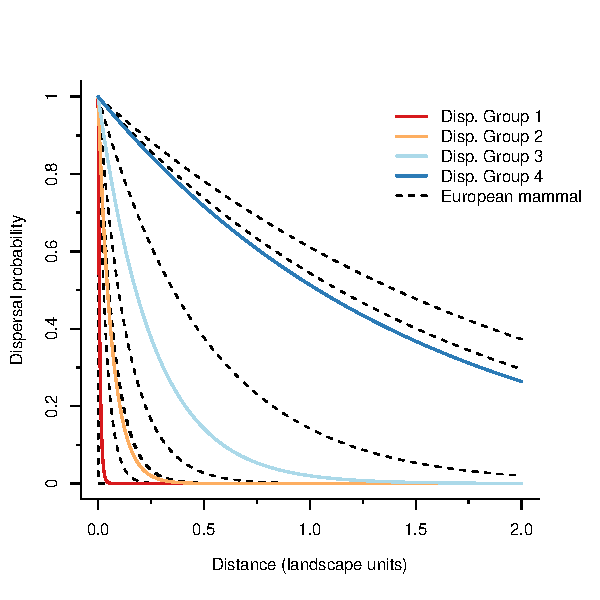
\includegraphics[width=6in]{../Figures/PlotWithLegendsMini.pdf}
\end{center}
%\caption{
%{\bf Bold the first sentence.}  Rest of figure 2  caption.  Caption 
%should be left justified, as specified by the options to the caption 
%package.
%}
%\label{Figure_label}
\end{figure}

\clearpage


%%-------------------
%\begin{figure}
%\begin{subfigure}{.5\textwidth}
%  %\centering
%  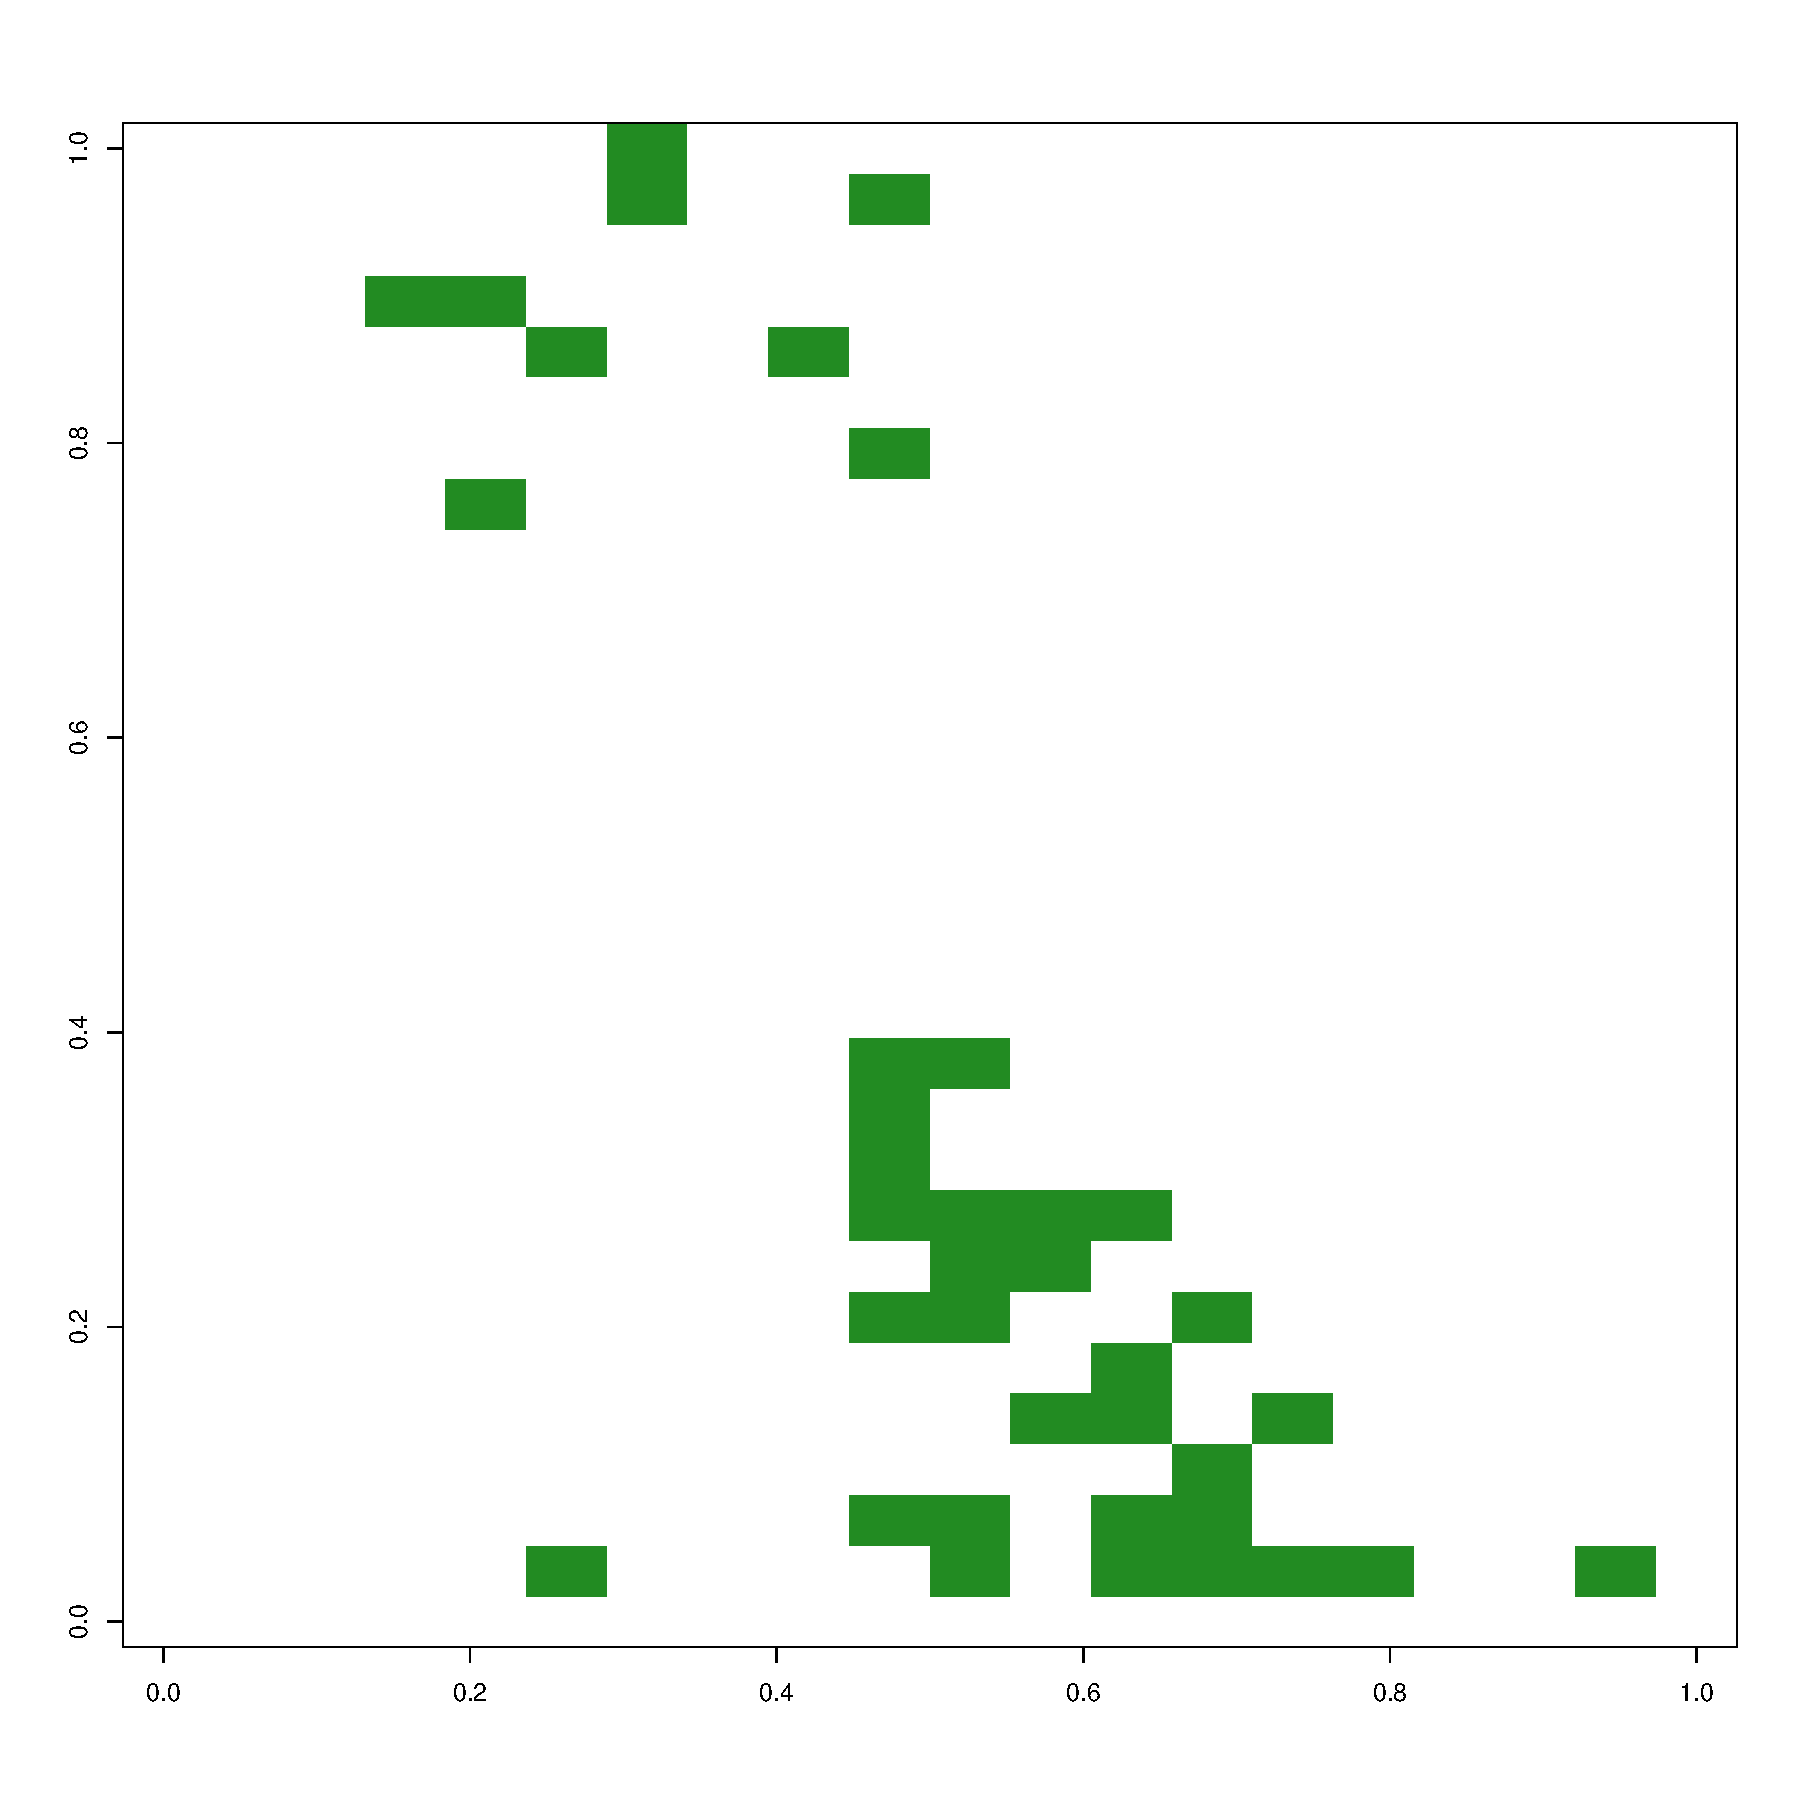
\includegraphics[width=6cm]{../Figures/v188_188_matrixpic.pdf}
%  \caption{1a}
%  \label{fig:sfig1}
%\end{subfigure}%
%\begin{subfigure}{.5\textwidth}
%  %\centering
%  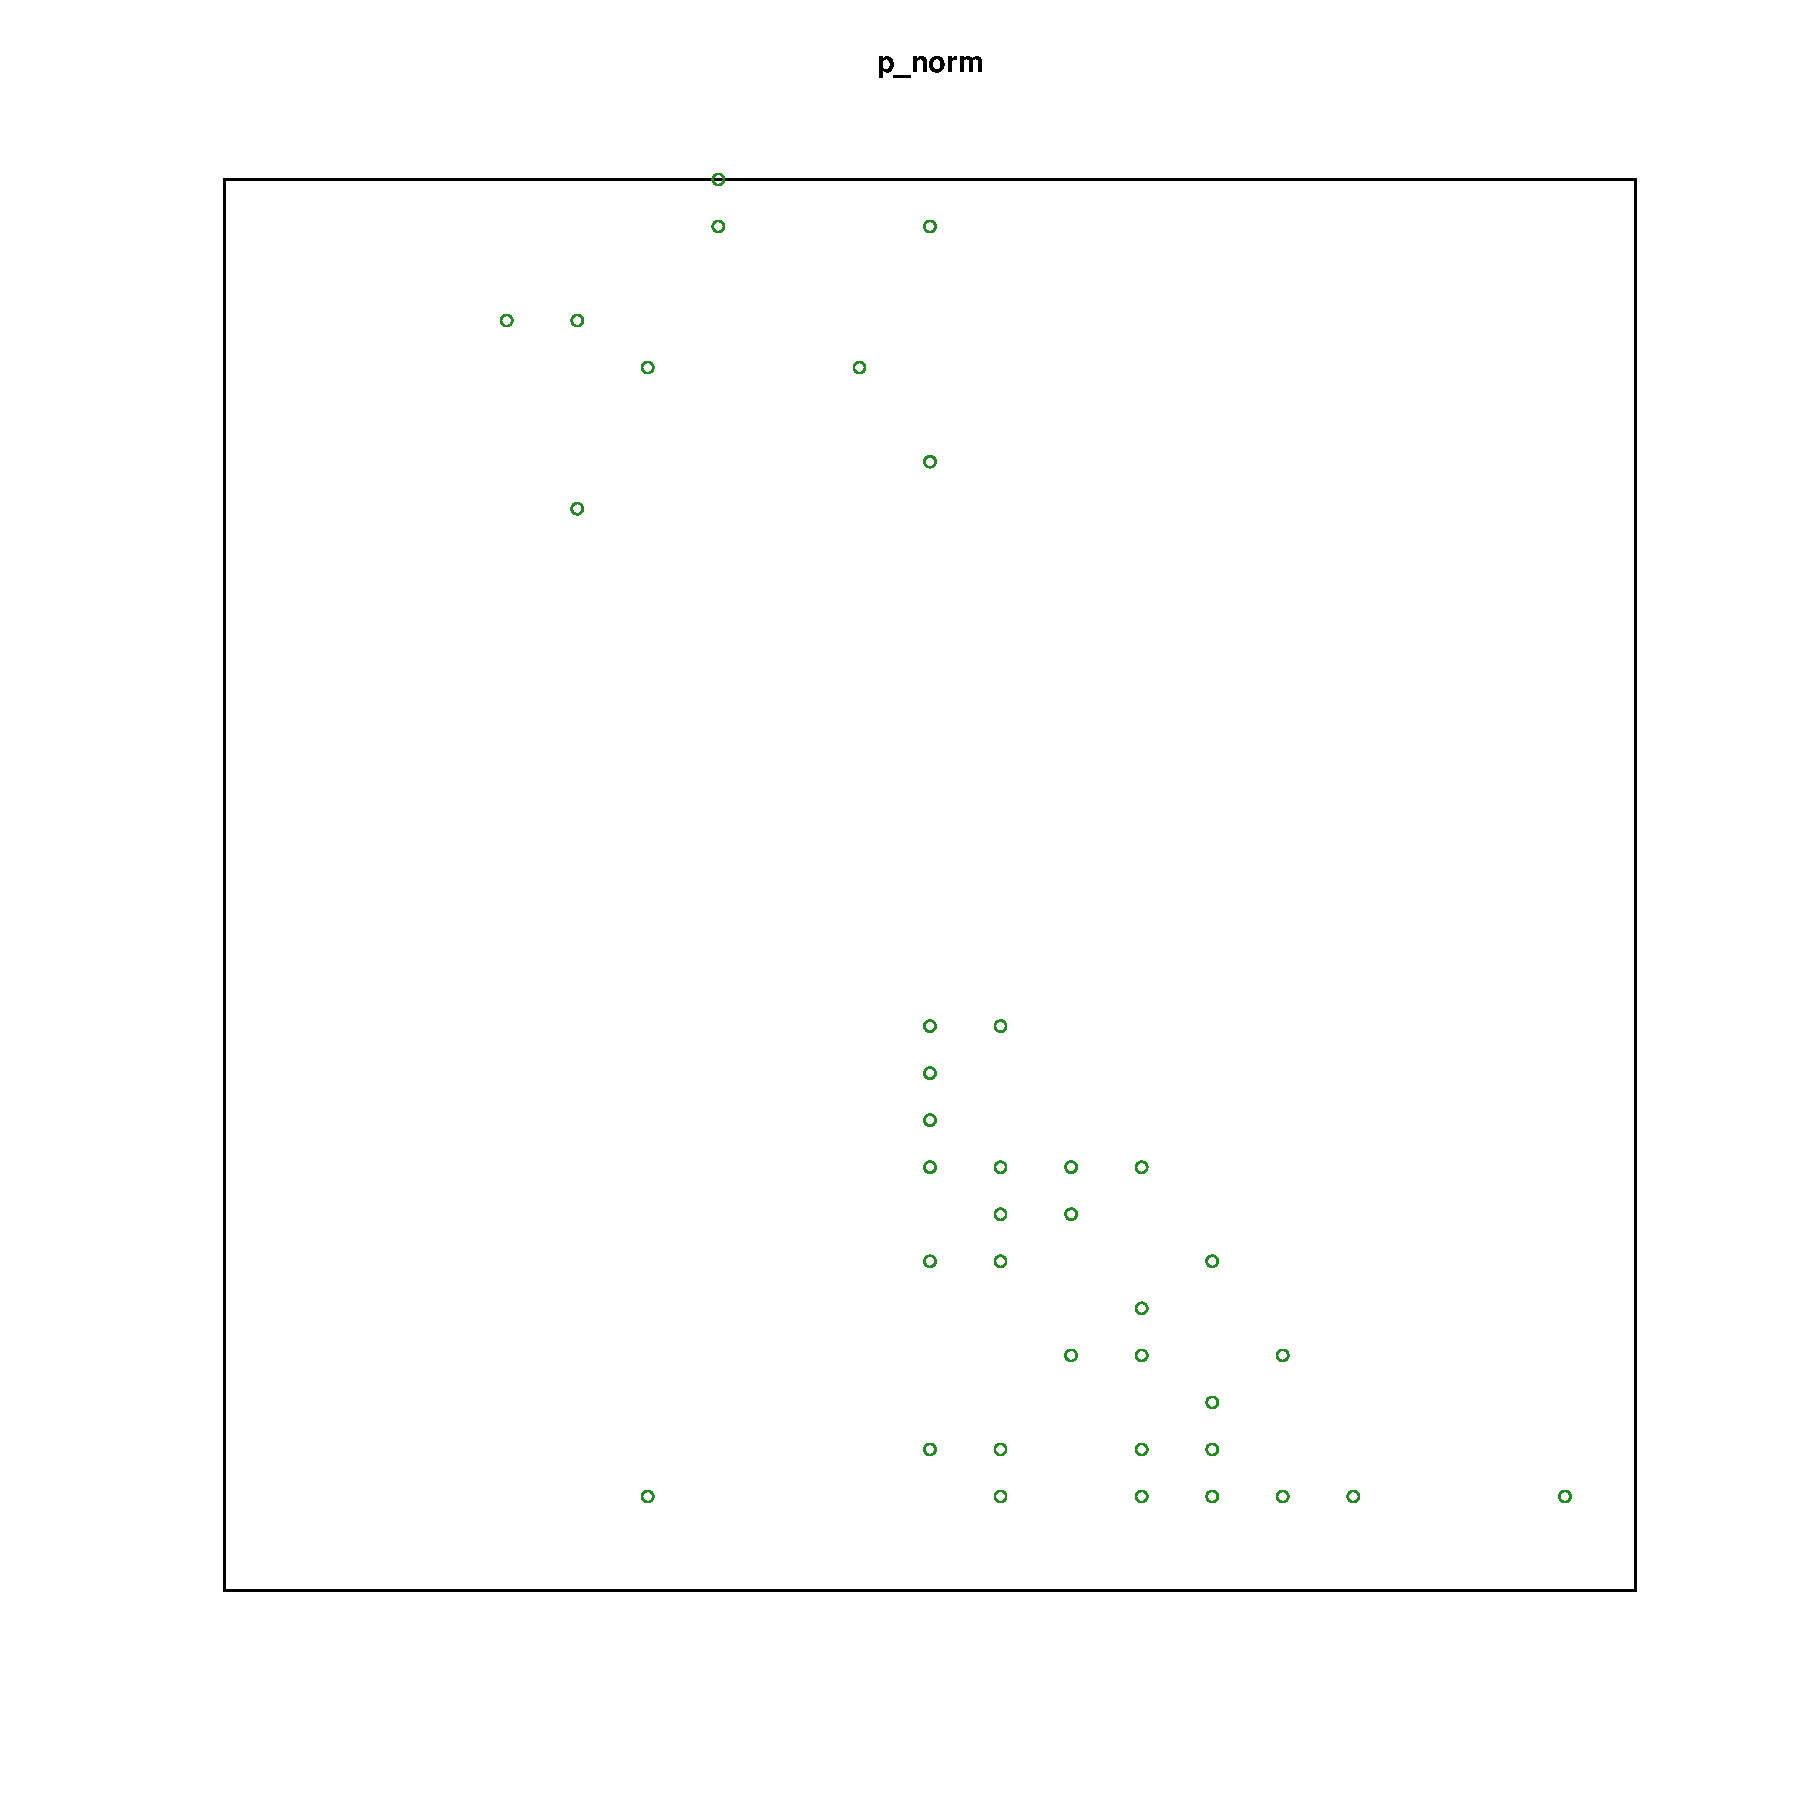
\includegraphics[width=6.75cm]{../Figures/v188_188_pnorm.pdf}
%  \caption{1b}
%  \label{fig:sfig2}
%\end{subfigure}
%\caption{plots of....}
%\label{fig:fig}
%\begin{subfigure}{.5\textwidth}
%  %\centering
%  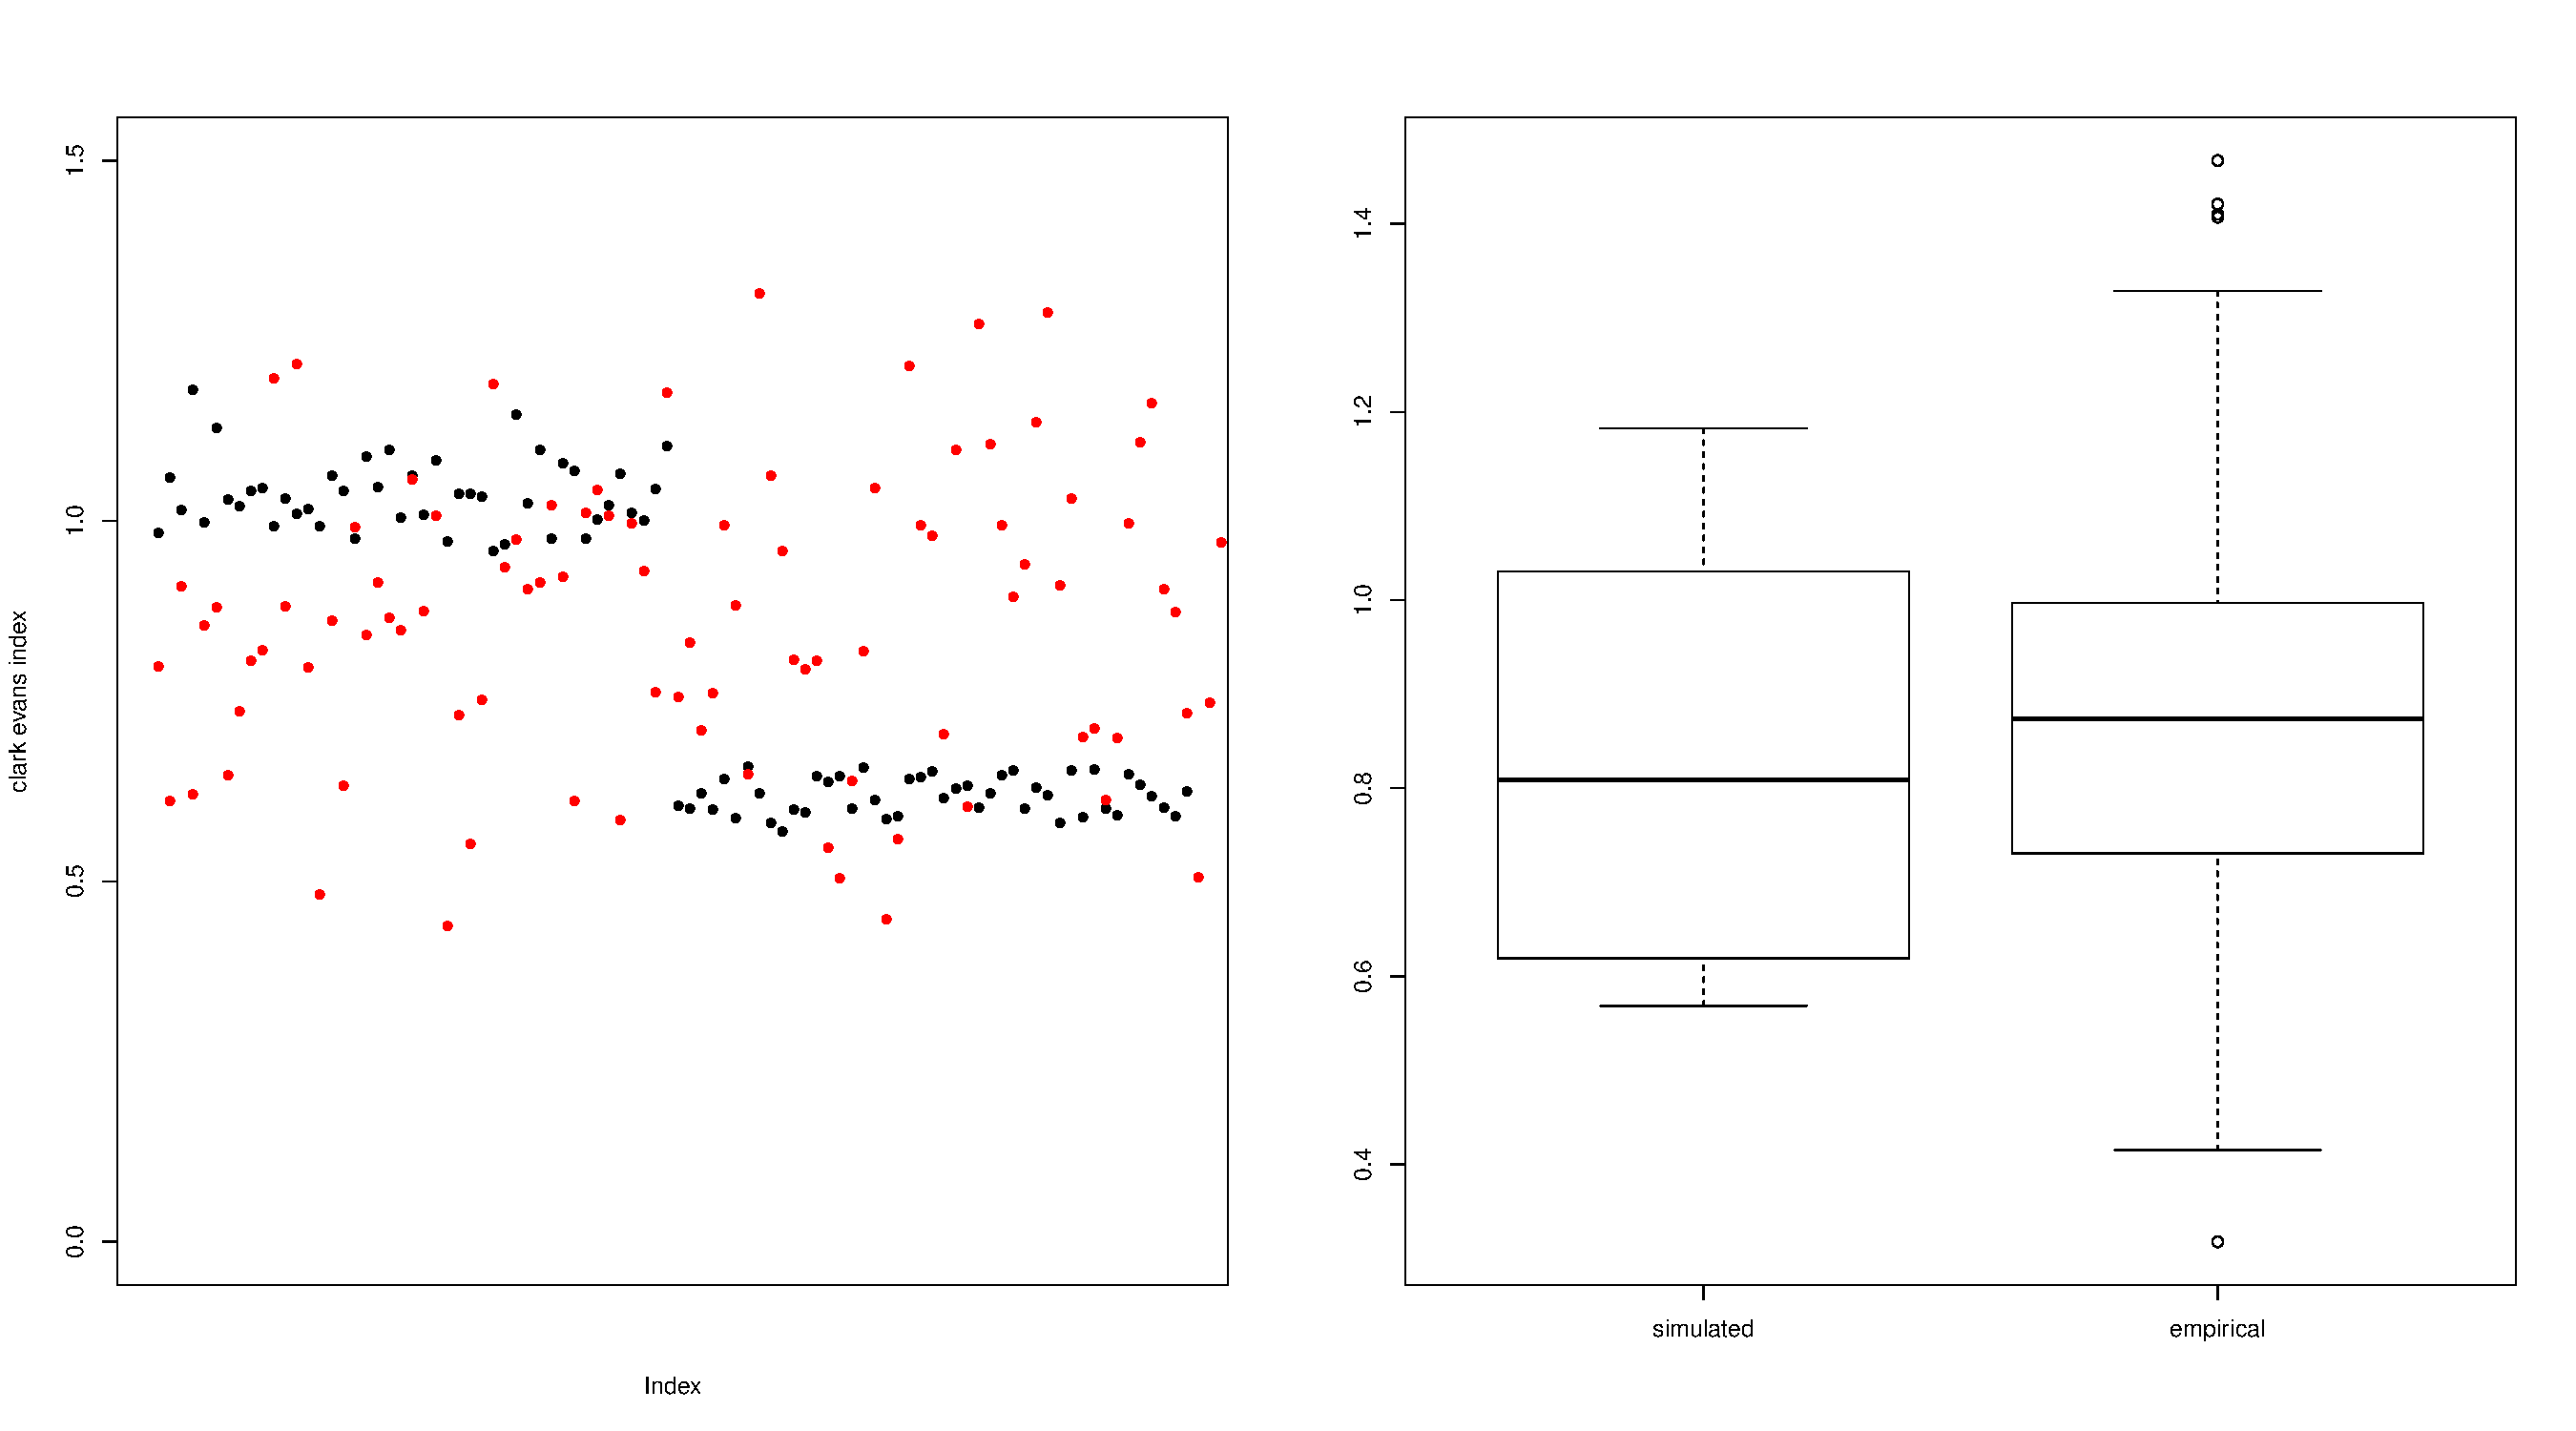
\includegraphics[width=12.75cm]{../Figures/SummaryFigure.pdf}
%  \caption{1b}
%  \label{fig:sfig3}
%\end{subfigure}
%\caption{plots of....}
%\label{fig:fig}
%\end{figure}
%%------------------

\clearpage

\begin{figure}[!ht]
\begin{center}
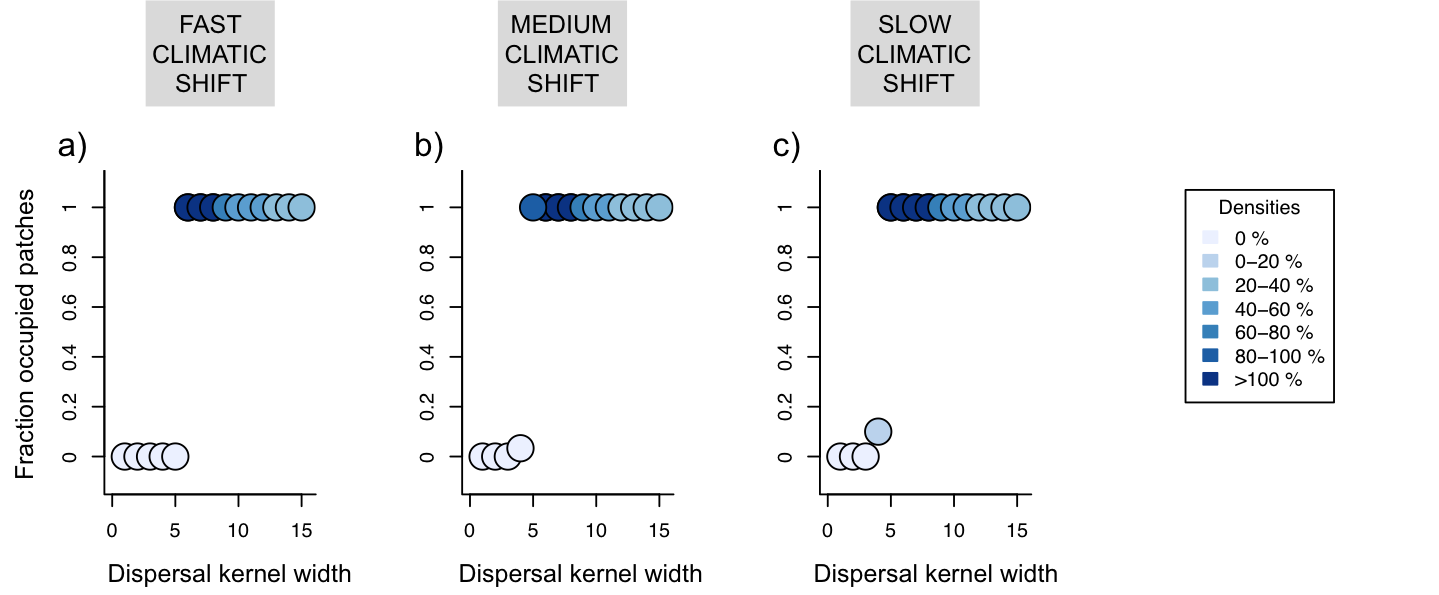
\includegraphics[width=7in]{../Figures/homo.png}
\end{center}
\end{figure}

\begin{figure}[!ht]
\begin{center}
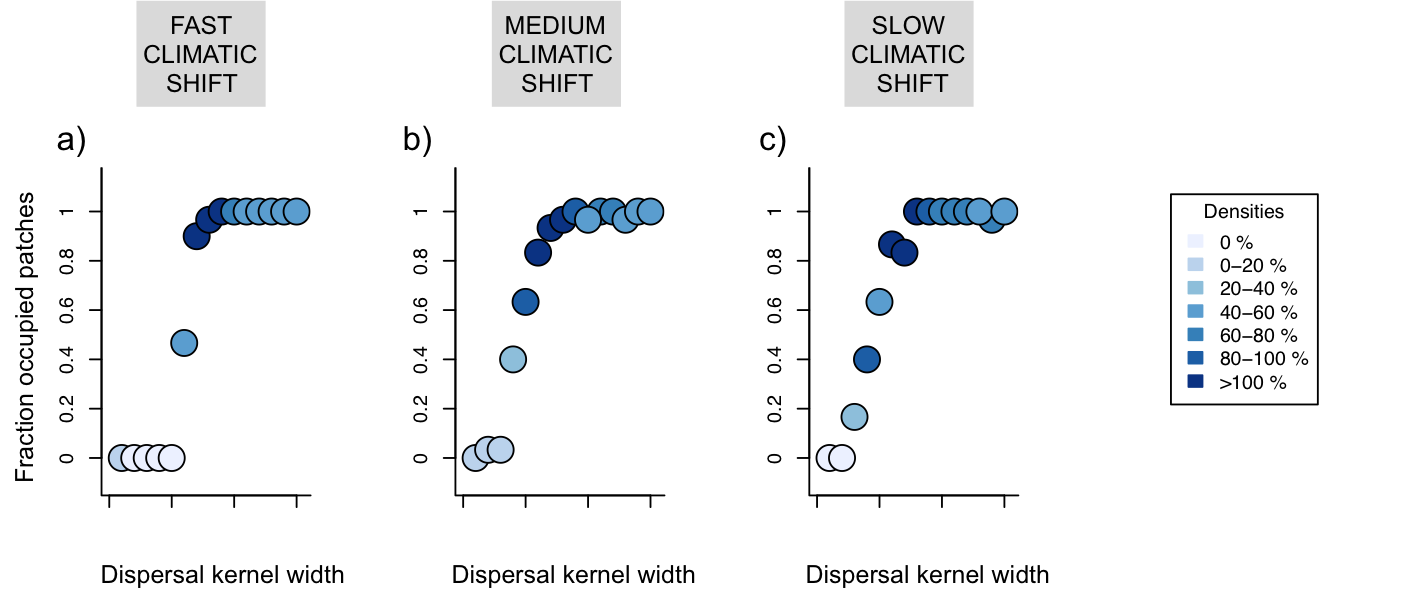
\includegraphics[width=7in]{../Figures/hetero.png}
\end{center}
\end{figure}

\clearpage
%\begin{sidewaysfigure*}
\begin{figure}[!ht]
\begin{center}
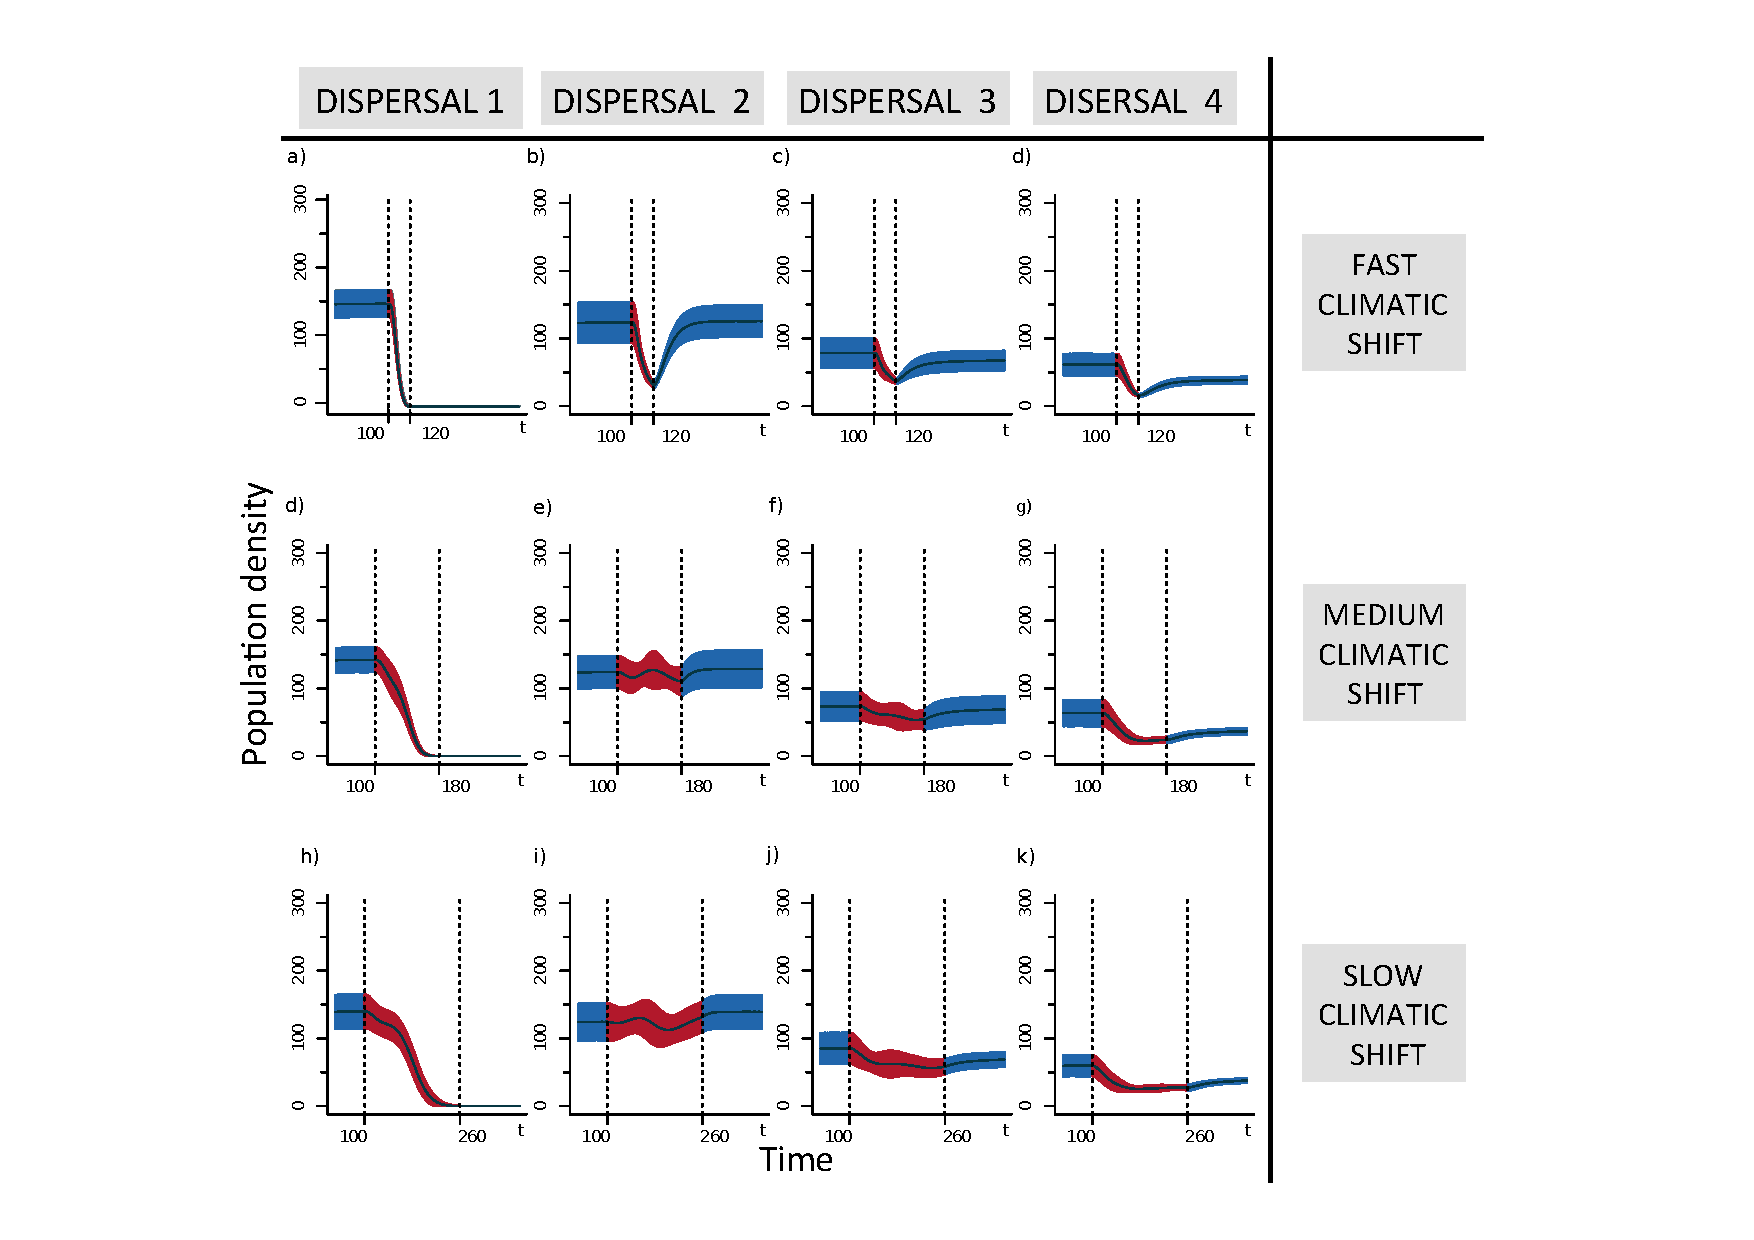
\includegraphics[width=8in]{../Figures/DensityFigHomo.pdf}
\end{center}
\end{figure}

\clearpage
%\begin{sidewaysfigure*}
\begin{figure}[!ht]
\begin{center}
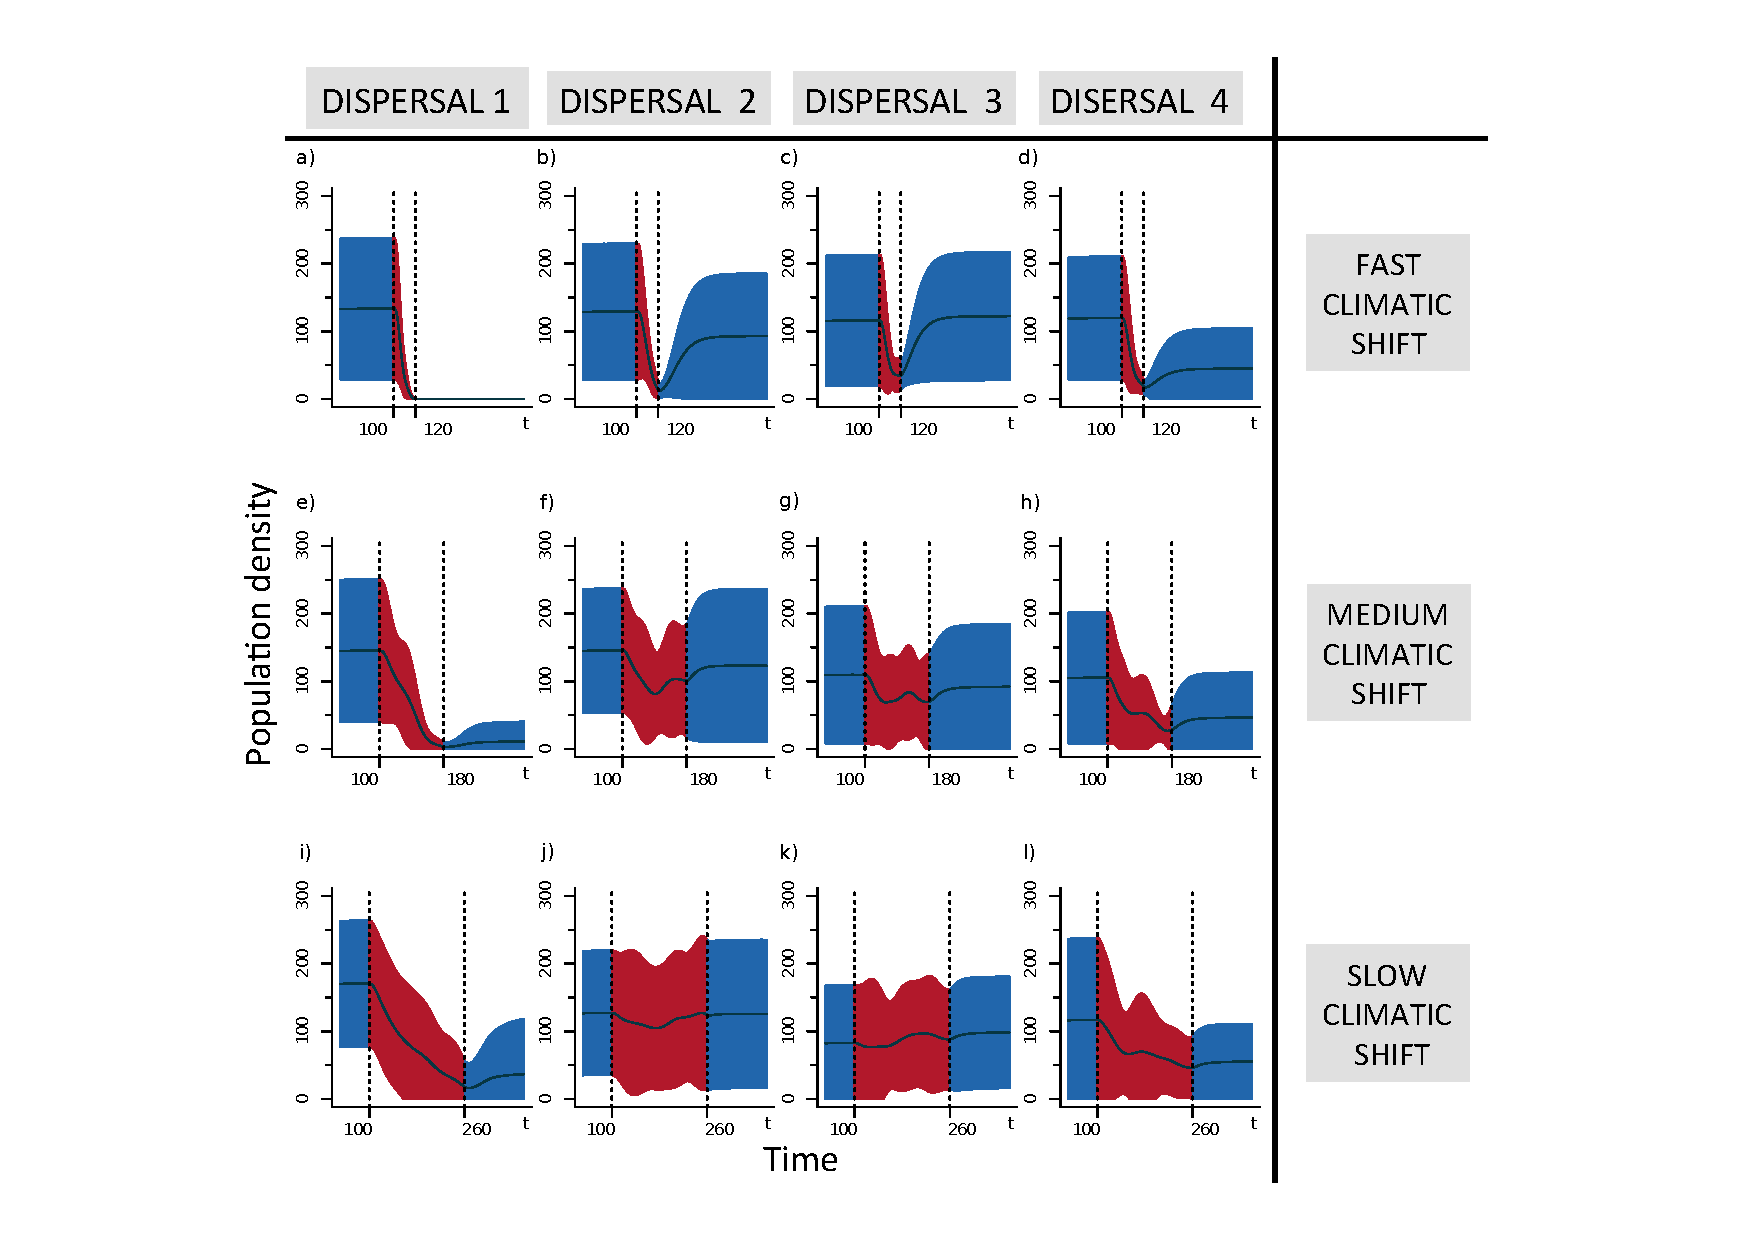
\includegraphics[width=8in]{../Figures/DensityFigHetero.pdf}
\end{center}
\end{figure}

\clearpage
\begin{table}
\begin{tabular}{lllll}
\hline
{\bf Split}						&{\bf Factor} 						&{\bf Number obs.} 					 	&{\bf Mean \# occ. patches} 	\\	%&{\bf Mean}
\hline
\hline
\hspace{0.00cm}	0) 			&Root 	(all data)					&720 											&399\\ 			%&3.85e+07 

\hspace{0.4cm}	1) 			&DispGroup =1 					&180 										 	&32  \\		%&1.77e+06 

\hspace{0.8cm}  2) 				&LandscapeType=2,6A,6B 			&152 										 	&16  \\		%&8.20e+05 

\hspace{1.6cm} 4) 				&LandscapeType=2 				&90 												&1 *\\		%&1.65e+03   

\hspace{1.6cm} 4) 				&LandscapeType=6A,6B 				&62 										  		&37  \\		%&7.71e+05

\hspace{3.2cm} 8) 				&Simlength $<$ 120 				&39 										  		&12 *\\		%&9.17e+04

\hspace{3.2cm} 8) 				&Simlength $\geq$120 				&23 										  		&79 *\\		%&6.14e+05
	
\hspace{0.8cm} 2) 				&LandscapeType=6C 				&28 										 		&119  \\		%&6.98e+05

\hspace{2cm} 5) 				&Simlength$<$ 50 					&14 										  		&0.1 *\\		%&9.28e-01 

\hspace{2cm} 5) 				&Simlength$\geq$50 				&14 									 			&238 *\\		%&3.01e+05

\hspace{0.4cm} 1) 				&DispGroup=2,3,4 					&540 										 	&521  \\		%&4.46e+06

\hspace{1.2cm} 3) 				&DispGroup=2 					&180 											&465  \\		%&2.64e+06 

\hspace{2.4cm} 6) 				&LandscapeType=6A,6B 				&64 										 		&410 *\\		%&2.25e+06

\hspace{2.4cm} 6) 				&LandscapeType=2,6C 				&116 									 		&494 *\\		%&9.58e+04

\hspace{1.2cm} 3) 				&DispGroup=3,4 					&360 											&549  \\		%&9.65e+05 
	
\hspace{2.8cm} 7) 				&DispGroup=3 					&180 										 	&532 *\\		%&1.83e+05

\hspace{2.8cm} 7)				&DispGroup=4 					&180											&566 *\\		%&6.80e+05 
\hline
\end{tabular}
\caption{Regression tree explaining the number of patches occupied at the end of the simulation. Entities with * indicate terminal branches.}
\end{table}

\begin{table}
\begin{tabular}{lllll}
\hline
{\bf Split}										&{\bf Factor} 						&{\bf Number obs.} 			&{\bf Mean pop. density} 	\\ %&{\bf Mean} 		
\hline
\hline
\hspace{0.00cm}	0)						&Root 	(all data)				&720 							 	&45056 \\ 	%&2.281378e+12 
\hspace{0.4cm}   1) 							&DispGroup=1,4 				&360 							  	&19086\\ 	%&3.660363e+11
 \hspace{0.8cm}    2) 						&DispGroup=1 				&180 					   			&3616 *\\		%&5.420598e+10
   \hspace{0.8cm}  2) 						&DispGroup=4 				&180 							 	&34555\\	%&2.256819e+11 
  \hspace{1.6cm}    4) 						&LandscapeType=2,6B,6C 		&147 							 	&26973*\\	%&5.614345e+10 
   \hspace{1.6cm}	4) 						&LandscapeType=6A 			&33 								 	&68329\\	%&1.234460e+11 
     \hspace{2.4cm}   6) 						&Simlength$<$ 120 			&20 								  	&43689*\\	%&4.332136e+10
        \hspace{2.4cm}	6) 					&Simlength$\geq$120 			&13 								 	&106236*\\	%&4.930196e+10
\hspace{0.4cm}   1) 							&DispGroup=2,3 				&360 							  	&71026 \\	%&1.429732e+12
 \hspace{1.2cm}    3) 						&Simlength$<$ 50 				&120 							  	&28767*\\	%&2.724214e+10
   \hspace{1.2cm}  3) 						&Simlength$\geq$50 			&240 							  	&92156 \\	%&1.081035e+12
     \hspace{2.0cm} 5) 						&DispGroup=3 				&120 							  	&67534 \\	%&3.352959e+11
   \hspace{2.8cm}     7)						&LandscapeType=2,6C 			&73 								  	&55537*\\	%&2.080666e+10
       \hspace{2.8cm} 7)						&LandscapeType=6A,6B 			&47 								 	&86167*\\	%&2.876636e+11
     \hspace{2.0cm} 5) 						&DispGroup=2 				&120 							 	&116778 *\\	%&6.002396e+11
\hline
\end{tabular}
\caption{Regression tree explaining the global population density at the end of the simulation. Entities with * indicate terminal branches. }
\end{table}

\clearpage
%\begin{sidewaysfigure*}
\begin{figure}[!ht]
\begin{center}
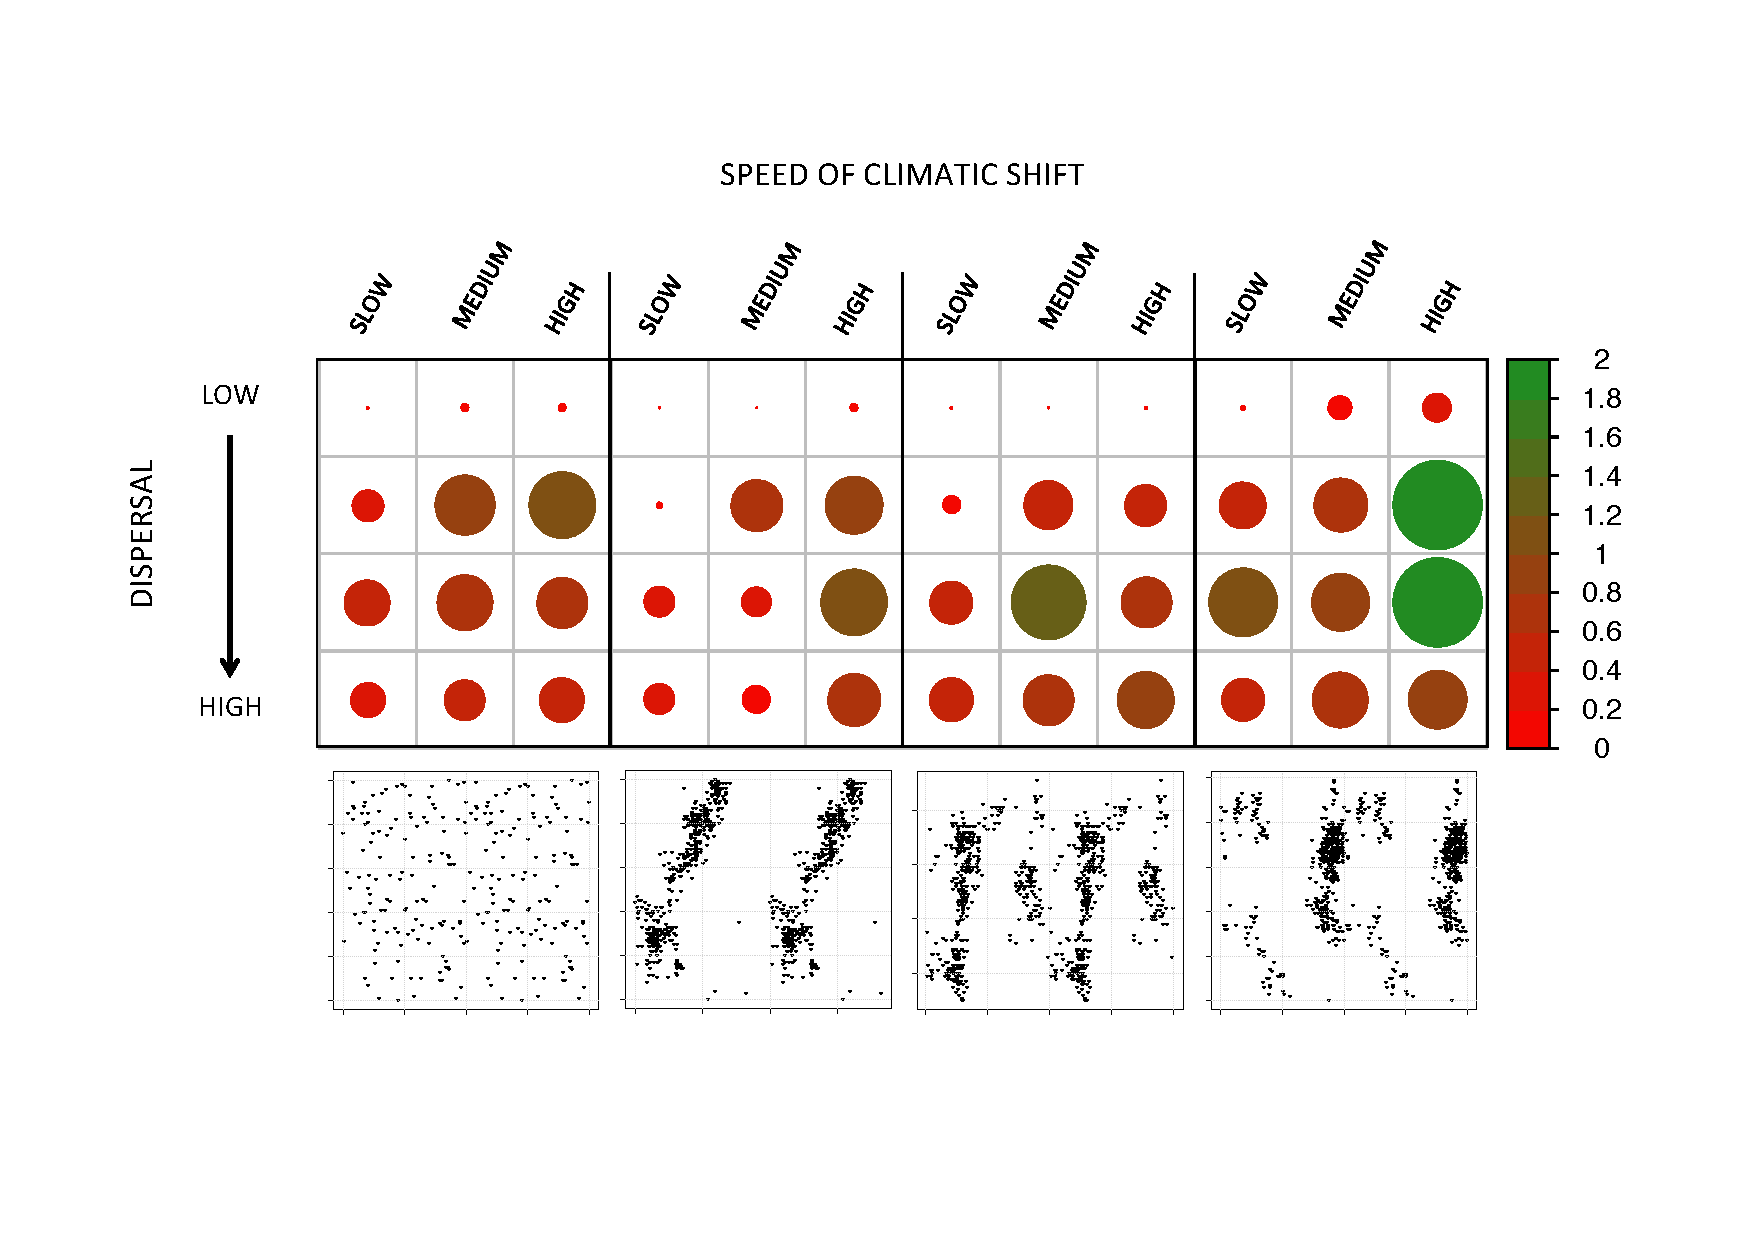
\includegraphics[width=8in]{../Figures/SummaryFigureConservation.pdf}
\end{center}
\end{figure}

\end{document}

